\chapter{Background}
\label{chap:background}

Before introducing the serverless paradigm,
we must understand what is cloud computing~\cite{nist}.
Despite its modern connotations, cloud computing
isn't a novel concept, in fact, its principles have been established
several decades ago: in essence, cloud computing
runs different types of workloads within clouds, which are environments that abstract, pool,
and share scalable resources across distributed networks.
Thus, users are offered on-demand availability of computing power by a third-party provider,
without the problems associated with direct active management of IT infrastructures.

\section{Cloud services}

Cloud computing is supplied as a collection of service models,
hence, users can arrange different abstraction layers based on their necessities.

\begin{enumerate}
  \item Infrastructure as a service (IaaS): these are the most low-level services that can be provided,
    like bare metal servers, storage, virtual machines, load balancers, etc.
  \item Platform as a service (PaaS): an entire toolkit or development environment
    made for scaling applications without thinking about the underlying infrastructure.
    PaaS vendors may offer programming languages execution environments, databases,
    web servers and many more technologies.
  \item Software as a service (SaaS): this model is in direct contact with the end-user,
    as it refers to the application software standing on top of the platforms and infrastructure.
    Cloud users, such as people using mobile phones, access the software through a subscription fee,
    without ever needing to install anything because the application is built on top of and balanced through
    the previously mentioned layers.
\end{enumerate}

Most recently, a new model has appeared, named FaaS--Function as a service,
delivering a cloud platform that offers computing runtimes with support for serverless architectures.

Furthermore, the serverless model is also encompassed as BaaS--Backend as a service,
usually accessible via APIs, providing support for many technologies like serverless databases,
but these services will not be examined in this thesis.

\section{Serverless computing}

Serverless computing was born due to a very pragmatic reason:
workloads in modern applications need to be efficiently managed
because they are highly dynamic, meaning that, some software parts
need more computing resources than the others and this aspect may vary frequently.
In traditional monoliths, or even microservices, developers are concerned
with capacity planning, configurations, management, fault tolerance, and
scaling containers, VMs or physical servers.

Serverless architectures abstract way all these inconveniences
by allowing developers to focus solely on writing application logic,
and letting the FaaS vendors to handle the burden of provisioning and scaling infrastructures.

To achieve this goal, developers write the logic inside computational units
called cloud functions, which are run in short-lived environments triggered by some kind of event.
Cloud functions recall the concept of programming languages functions,
as they both associate an input to an output, and as a matter of fact, 
cloud functions' logic is encapsulated inside the latter.
Yet, cloud functions need to be considered as resources rather than instructions of code,
as they are computing units invoked by the serverless provider and metered on-demand through an event-driven execution model,
thus they can be written in different programming languages (e.g., \textit{Go}, \textit{Java}, \textit{JavaScript})
as long as the chosen vendor has adequate support for the language runtime.

When the cloud function is triggered by an event such as
HTTP requests, database changes, file uploads, scheduled intervals or various other triggers,
the FaaS provider runs the code
after initializing an execution environment, which is a secure and isolated context
that manages all the resources needed for the function lifecycle.
Execution environments are technically handled differently by the platform providers, for example,
\textit{AWS Lambda} uses $\mu$VMs while \textit{IBM} uses \textit{Docker} containers,
nonetheless they all offer lightweight sandboxed containers designed to
have fast startup/shutdown times and minimal overhead due to their virtualized nature.

% TODO: replace this image
\begin{figure}[H]
  \centering
  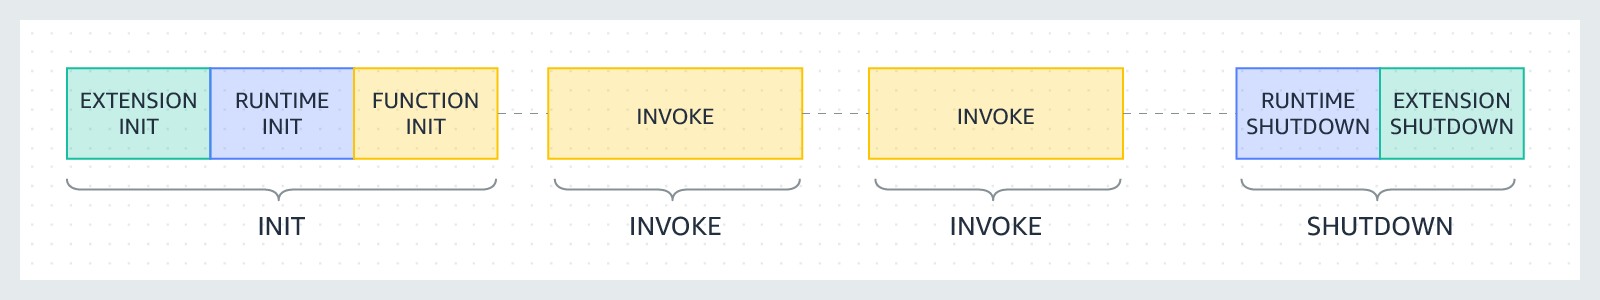
\includegraphics[width=\textwidth]{diagrams/lambda.png}
  \caption{Serverless function lifecycle in an execution environment.}
  \label{fig:serverless-functions-lifecycle}
\end{figure}

\subsection{Serverless principles}

Serverless is a misnomer, since servers are still in the picture,
this computing model must not be confused with other paradigms
that do not require an actual server such as peer-to-peer (P2P)~\cite{serverless-wikipedia}.
Instead, it is more accurate to interpret it as "less-server",
therefore emphasizing the shift in architectural responsibility from developers actively
managing server infrastructure to entrusting platform providers to manage the underlying server complexities.

Figure~\ref{fig:serverless-functions-lifecycle} shows that serverless functions
are ephemeral, so they are designed to have a temporary nature, and consequently
stateless, so there is no stored information of previous transactions, as they are constructed
from scratch each time they are instantiated.
These behaviors have several implications that may offer advantages and disadvantages.

\subsubsection{Serverless architectures benefits}

\paragraph{\textbf{Reduced costs}} Serverless at its core gives immediate
business value to its users, because it outsources servers management
to a vendor, also allowing for economies of scale to take place, as discussed in \cite{berkeley}.
Operational expenses decrease significantly, and development costs are optimized
since this cloud paradigm offers the most fine-grained billing model in which developers
only pay for the actual functions' execution time and not for idle servers.

\paragraph{\textbf{Elasticity}} The cloud provider is responsible for autoscaling the capacity
on demand, hence resources are handled accordingly to accommodate the required load.
For example, consider a web application with two HTTP endpoints, denoted as endpoint $A$ and endpoint $B$,
where $A$ is frequently called while $B$ is very rarely requested.
In a traditional monolith, the entire web app would need to manually be scaled
to handle unpredictable load spikes of $A$ calls, and even in normal circumstances
the costs would still be inefficiently allocated just to manage some occasional $B$ requests.
By encapsulating their logic inside two different serverless functions,
endpoint $A$ can be allocated more resources when it experiences high demand,
while endpoint $B$ might cost almost zero due to its occasional requests.

\paragraph{\textbf{Productivity}} Developers can focus solely on writing
business logic. Exposing units of code only through an event-driven model simplifies back-end development,
also alleviating the typical problems related to distributed systems (e.g., multithreading).
Moreover, development becomes quicker as deploying is easier and updates are granular,
thus increasing the agility of the team and rapid prototyping of new products.

\paragraph{\textbf{High availability}} Thanks to the distributed nature of serverless computing,
platform providers ensure fault tolerance by redirecting functions across healthy and available zones.
Latency is also reduced by deploying functions geographically near the end-users.

\paragraph{\textbf{Interoperability}} The serverless paradigm can be used in
conjunction with code deployed in traditional styles,
such as microservices or monoliths~\cite{serverless-wikipedia}.
Therefore, this model can be incrementally adopted by large companies and benefit
complex existing systems. Start-ups should prioritize following a pure serverless approach
because of all the previously mentioned benefits.

\subsubsection{Serverless architectures shortcomings}

Serverless computing is not flawless, and some researchers \cite{two-steps-back}
point out the limits that are inherent to this paradigm, which cannot be solved
by updating the state of the art with tools like \f{} itself.

\paragraph{\textbf{State management}} Considering that there is no server-state,
the programming model needs to shift for developers, as numerous applications require
storing data for future references.
To limit this disadvantage, users may use:
\begin{itemize}
  \item Temporary data stores or distributed caches, like Redis.
  \item Databases, both SQL or NoSQL, as long as the connections can be instantiated quickly.
  \item Vendor-specific strategies, like \textit{AWS}' step functions or \textit{Azure}'s durable functions.
\end{itemize}
Also, the limited lifetime of serverless functions needs to be contemplated given that
they are not designed to support long-running processes,
and if misused they can become more costly than traditional solutions.

\paragraph{\textbf{Cold starts}} Serverless functions startup times
can be a crucial drawback for systems performance, as the overhead for
allocating all the resources needed to run a function can cause significant
delays. This well-known problem, named "cold start", is
particularly emphasized with technologies requiring heavy runtimes, such as JVM-based languages.
To avoid this constraint, platform providers usually wait some time
before dismantling the container, keeping it in a so-called "warm" state,
so they are able to run the code without all the initialization overhead:
this approach is obviously more costly, but it dramatically improves performances.

\paragraph{\textbf{Vendor lock-in}}

\subsection{Serverless use cases}

Lorem ipsum dolor sit amet, qui minim labore adipisicing minim sint cillum sint consectetur cupidatat.
Parlare anche del framework serverless

\section{Server-side JavaScript}

Lorem ipsum dolor sit amet, qui minim labore adipisicing minim sint cillum sint consectetur cupidatat.

\subsection{TypeScript}

Lorem ipsum dolor sit amet, qui minim labore adipisicing minim
